\documentclass[fr]{../../../../../../eplexam}

\usepackage{diagbox}

\hypertitle{Gestion de production et des opérations}{5}{ECGE}{1223}{2013}{Janvier}
{Florian Thuin\and Aymeric de Cocq}
{Pierre Semal}

\section{}
 Votre entreprise a la possiblité de fabriquer et de vendre 5 produits numérotés de 1 à 5. \newline
 
 Il s'agit de nouveaux produits qui utiliseraient 3 machines indépendantes que vous n'utilisez plus aujourd'hui. Ces machines sont nommés A, B et C. Ces machines peuvent fonctionner automatiquement. Sur une pause normale de 8h (un shift), il faut déduire 2 heures pour les temps de chargement, de démarrage et d'entretien. Vous travaillez actuellement avec une seule pause par jour, soit 6 heures de travail efficace sur chaque machine. \newline
 
 Le tableau suivant reprend le temps nécessaire à chaque machine pour la fabrication de chaque produit. Ainsi, par exemple, le produit 1 requiert 1 minute de travail à la machine A et ensuite 2 minutes de travail à la machine B et 4 minutes à la machine C. \newline
 
 \noindent
 \begin{tabular}{|l|c|c|c|c|c|}
  \hline
  \diagbox{Ateliers}{Produits} & Produit 1 & Produit 2 & Produit 3 & Produit 4 & Produit 5 \\
  \hline
  Atelier A & 1 & 2 & 3 & 0 & 3 \\
  \hline
  Atelier B & 2 & 2 & 3 & 3 & 2 \\
  \hline
  Atelier C & 4 & 3 & 0 & 3 & 2 \\
  \hline
 \end{tabular} \medskip
 
 \paragraph{Question 1a} (4 points)
 Supposons que tous ces produits aient la même profitabilité et qu'il est aussi facile de les vendre les uns que les autres. Si vous souhaitez maximiser votre profitabilité, quel(s) produit(s) produiriez-vous et combien en vendriez-vous par jour ? \newline

\begin{solution}

%  Pour maximiser son profit, il faut maximiser la quantité produite (notée q) par rapport au prix (noté p) :
 
%  \[
%   \textrm{max } P_{1}*Q_{1} + P_{2}*Q_{2} + P_{3}*Q_{3} + P_{4}*Q_{4} + P_{5}*Q_{5}
%  \]

%  Puisque tous les prix sont égaux, on peut les normaliser à 1 et on devra maximiser leur quantité.
 
%  \[
%   \textrm{max } Q_{1} + Q_{2} + Q_{3} + Q_{4} + Q_{5}
%  \]
 
 Le plus facile puisqu'il n'y a pas beaucoup de produits est de réaliser un raisonnement inductif, en faisant des mix de 1 à 5 produits.
 
 Le raisonnement est simple : on est limité par le temps de production maximal sur la chaîne \newline


  \noindent
 \begin{tabular}{|l|c|c|c|c|c|}
  \hline
  \diagbox{Ateliers}{Produits} & Produit 1 & Produit 2 & Produit 3 & Produit 4 & Produit 5 \\
  \hline
  Atelier A & 1 & 2 & 3 & 0 & 3 \\
  \hline
  Atelier B & 2 & 2 & 3 & 3 & 2 \\
  \hline
  Atelier C & 4 & 3 & 0 & 3 & 2 \\
  \hline
  \rowcolor{red!60} Temps maximum & 4 & 3 & 3 & 3 & 3 \\
  \hline
 \end{tabular} \medskip
 

 Sachant qu'il y a 6 heures de travail efficace (360 minutes) par machine par jour, on que les chiffres du tableau sont exprimés en minutes, il suffit de faire une règle de 3 pour trouver le niveau de production.
 
 Cependant, intuitivement en voyant les temps de production, on peut déjà conclure que le produit 1 sera plus long à produire que les autres et sera donc inintéressant dans le cas où on ne souhaite produire qu'un seul type de produit. \newline
 

  \noindent
 \begin{tabular}{|l|c|c|c|c|c|}
  \hline
  \diagbox{Ateliers}{Produits} & Produit 1 & Produit 2 & Produit 3 & Produit 4 & Produit 5 \\
  \hline
  Atelier A & 1 & 2 & 3 & 0 & 3 \\
  \hline
  Atelier B & 2 & 2 & 3 & 3 & 2 \\
  \hline
  Atelier C & 4 & 3 & 0 & 3 & 2 \\
  \hline
  \rowcolor{red!60} Temps maximum & 4 & 3 & 3 & 3 & 3 \\
  \hline
  \rowcolor{red!60} Productivité journalière & 90 & 120 & 120 & 120 & 120 \\
  \hline
 \end{tabular} \medskip
 
  La productivité maximale avec un produit est donc de 120 unités par jour, pour les produits 2, 3, 4 et 5.
 

 Si nous augmentons et souhaitons produire 2 produits, les choix qui s'offrent à nous sont les suivants : 1 + 2 ; 2 + 3 ; 3 + 4 ; 4 + 5 ; 1 + 3 ; 1 + 4 ; 1 + 5 ; 2 + 4 ; 2 + 5 : 3 + 5. \newline
 

  \noindent
 \small \begin{tabular}{|l|c|c|c|c|c|c|c|c|c|c|}
  \hline
  \diagbox{Ateliers}{Produits} 	& 1 + 2	& 2 + 3	& 3 + 4 & 4 + 5 & 1 + 3 & 1 + 4 & 1 + 5 & 2 + 4 & 2 + 5 & 3 + 5 \\
  \hline
  Atelier A 			& 3 	& 5 	& 3 	& 3 	& 4	& 1	& 4	& 2	& 5 	& 6\\
  \hline
  Atelier B 			& 4 	& 5 	& 6 	& 5 	& 5	& 5	& 4	& 5 	& 4	& 5\\
  \hline
  Atelier C 			& 7 	& 3 	& 3 	& 5 	& 4	& 7	& 6	& 6 	& 5 	& 2\\
  \hline
  \rowcolor{red!60} Temps maximum & 7 	& 5 	& 6 	& 5 	& 5	& 7	& 6	& 6 	& 5 	& 6\\
  \hline
  \rowcolor{red!60} Productivité journalière & 102,86 & 144 & 120 & 144 & 144 & 102,86 & 120 & 120 & 144 & 120 \\
  \hline
 \end{tabular} \medskip
 

 La productivité maximale avec deux produits s'élèvent à 144 produits par jour pour les mix 2 + 3, 4 + 5, 1 + 3, 2 + 5.
 
 Intéressons-nous maintenant à 3 produits. Les mélanges possibles sont : 1 + 2 + 3 ; 2 + 3 + 4 ; 3 + 4 + 5 ; 1 + 2 + 4 ; 1 + 2 + 5 ; 2 + 3 + 5. \newline
 

 \noindent
 \begin{tabular}{|l|c|c|c|c|c|c|}
  \hline
  \diagbox{Ateliers}{Produits} 	& 1 + 2 + 3 & 2 + 3 + 4 & 3 + 4 + 5 & 1 + 2 + 4 & 1 + 2 + 5 & 2 + 3 + 5 \\
  \hline
  Atelier A 			& 6 	    & 5 	& 6 	    & 3 	& 6	    & 8 \\
  \hline
  Atelier B 			& 7 	    & 8 	& 8 	    & 7 	& 6	    & 7 \\
  \hline
  Atelier C 			& 7 	    & 6 	& 5 	    & 10 	& 9	    & 5 \\
  \hline
  \rowcolor{red!60} Temps maximum & 7 	    & 8 	& 8 	    & 10 	& 9	    & 8 \\
  \hline
  \rowcolor{red!60} Productivité journalière & 154,28 & 135 & 135   & 108       & 120       & 135 \\
  \hline
 \end{tabular} \medskip
 
 La productivité maximale avec trois produits s'élèvent à 154,28 produits et la seule possibilité est de produire 1 + 2 + 3.
 
 Intéressons-nous maintenant à 4 produits. Les mélanges possibles sont : 1 + 2 + 3 + 4 ; 2 + 3 + 4 + 5 ; 1 + 2 + 4 + 5; 1 + 3 + 4 + 5 ; 1 + 2 + 3 + 5. \newline
 

 \noindent
 \begin{tabular}{|l|c|c|c|c|c|}
  \hline
  \diagbox{Ateliers}{Produits} 	& 1 + 2 + 3 + 4 & 2 + 3 + 4 + 5 & 1 + 2 + 4 + 5 & 1 + 3 + 4 + 5 & 1 + 2 + 3 + 5 \\
  \hline
  Atelier A 			& 6 	    	& 8 		& 6 	    	& 7		& 9 \\
  \hline
  Atelier B 			& 10 	    	& 10 		& 9 	    	& 10 		& 9 \\
  \hline
  Atelier C 			& 10 	   	& 8 		& 12 	    	& 9 		& 9 \\
  \hline
  \rowcolor{red!60} Temps maximum & 10 	    	& 10 		& 12 	    	& 10 		& 9 \\
  \hline
  \rowcolor{red!60} Productivité journalière & 144 & 144 	& 120   	& 144		& 160 \\
  \hline
 \end{tabular} \medskip
 
 La productivité maximale avec quatre produits s'élèvent à 160 produits et la seule possibilité est de produire 1 + 2 + 3 + 5.
 
 Intéressons maintenant à 5 produits. Le seul mélange possible est évidemment : 1 + 2 + 3 + 4 + 5. \newline
 

 \noindent
 \begin{tabular}{|l|c|}
  \hline
  \diagbox{Ateliers}{Produits} 	& 1 + 2 + 3 + 4 + 5 \\
  \hline
  Atelier A 			& 9 \\
  \hline
  Atelier B 			& 12 \\
  \hline
  Atelier C 			& 12 \\
  \hline
  \rowcolor{red!60} Temps maximum & 12 \\
  \hline
  \rowcolor{red!60} Productivité journalière & 150 \\
  \hline
 \end{tabular} \medskip
 
 La productivité maximal avec cinq produits s'élèvent à 150 produits et la seule possibilité est de produire 1 + 2 + 3 + 4 + 5.
 
 Il faut maintenant trouver la productivité maximale parmi tous les cas possibles. La meilleure solution est 160 produits par jour en produisant 1 + 2 + 3 + 5. Comme on sait que tous les produits sont vendus, on vendra donc 160 produits par jour.

\end{solution}


 \paragraph{Question 1b} (3 points)
 Votre réponse change-t-elle, et comment, si :
 \begin{enumerate}
  \item La profitabilité du produit 4 et de 50\% supérieure à celle des autres.
  \item La machine A est une machine de peinture qui applique une couche en une minute (donc, par exemple, 3 couches pour le produit 3) mais qui requiert 1 minute de séchage entre chaque couche. 
 \end{enumerate}

\begin{solution}

 Si la profitabilité du produit 4 est de 50\% supérieure à celle des autres, il faut recalculer la production de 1 produit 3 comme la production de 1,5 produit. 
 
 Voici les calculs pour les cas où le produit 4 est présent :
 \begin{itemize}
  \item $ 120 * P_{4}  * 1,5 = 180 $ produits
  \item $ 60 * P_{3} + 60 * P_{4} * 1,5 = 150 $ produits
  \item $ 72 * P_{4} * 1,5 + 72 * P_{5} = 180 $ produits
  \item $ 51,43 * P_{1} + 51, 43 * P_{4} * 1,5 = 128,58 $ produits
  \item $ 60 * P_{2} + 60 * P_{4} * 1,5 = 150 $ produits
  \item $ 45 * P_{2} + 45 * P_{3} + 45 * P_{4} * 1,5 = 157,5 $ produits
  \item $ 45 * P_{3} + 45 * P_{4} * 1,5 + 45 * P_{5} = 157,5 $ produits
  \item $ 36 * P_{1} + 36 * P_{2} + 36 * P_{4} * 1,5 = 126 $ produits
  \item $ 36 * P_{1} + 36 * P_{2} + 36 * P_{3} + 36 * P_{4} * 1,5 = 162 $ produits
  \item $ 36 * P_{2} + 36 * P_{3} + 36 * P_{4} * 1,5 + 36 * P_{5} = 162 $ produits
  \item $ 30 * P_{1} + 30 * P_{2} + 30 * P_{4} * 1,5 + 30 * P_{5} = 135 $ produits
  \item $ 36 * P_{1} + 36 * P_{3} + 36 * P_{4} * 1,5 + 36 * P_{5} = 162 $ produits
  \item $ 30 * P_{1} + 30 * P_{2} + 30 * P_{3} + 30 * P_{4} * 1,5 + 30 * P_{5} = 165 $ produits
 \end{itemize}
 
 On peut se rendre compte que dans beaucoup de cas, la productivité est maintenant supérieure à la productivité de base.
 
 Dans le cas de $P_4$ seul, on produit 120 produits et on peut atteindre une productivité équivalente à 180 produits.
 
 Dans le cas de $P_4$ et $P_5$, on produit 144 produits et on peut atteindre une productivité équivalente à 180 produits. \newline

 Si la machine A ajoute une minute entre chaque minute, tous les calculs changent puisque le temps sur cette machine double. Pour éviter ces situations, le mieux est d'établir un buffer, puisque la situation s'y prête vraiment bien.
\end{solution}

 \paragraph{Question 1c} (2 points)
 Supposez que vous organisiez les machines A, B et C en une ligne et que vous fabriquez les produits 3, 4 et 5 en alternance : 3,4,5,3,4,5,3,4,5, etc. Si vous ne placez aucun buffer, quelle productivité atteindrez-vous et pourquoi ? \newline

\begin{solution}
 On doit faire une Gantt Chart pour se rendre compte de la situation lorsqu'il est demandé de sortir en alternance 3 puis 4 puis 5 \textbf{dans cet ordre précis}.
 

 \noindent
 \begin{tabular}{|l|c|c|c|c|c|c|c|c|c|c|c|c|c|c|c|c|c|c|c|c|c|c|}
  \hline
  \diagbox{\tiny Ateliers}{\tiny Minutes} 	& 1 & 2 & 3 & 4 & 5 & 6 & 7 & 8 & 9 & 10 & 11 & 12 & 13 & 14 & 15 & 16 & 17 & 18 \\
  \hline
  Atelier A 			& \cellcolor{red!60}$P_{3}$ & \cellcolor{red!60}$P_{3}$ & \cellcolor{red!60}$P_{3}$ & & & & \cellcolor{green!60}$P_{5}$ & \cellcolor{green!60}$P_{5}$ & \cellcolor{green!60}$P_{5}$ & \cellcolor{red!60}$P_{3}$ & \cellcolor{red!60}$P_{3}$ & \cellcolor{red!60}$P_{3}$ & & & & \cellcolor{green!60}$P_{5}$ & \cellcolor{green!60}$P_{5}$ & ... \\
  \hline
  Atelier B 			&	&	&	 & \cellcolor{red!60}$P_{3}$ & \cellcolor{red!60}$P_{3}$ & \cellcolor{red!60}$P_{3}$ & \cellcolor{blue!60}$P_{4}$ & \cellcolor{blue!60}$P_{4}$ & \cellcolor{blue!60}$P_{4}$ & \cellcolor{green!60}$P_{5}$ & \cellcolor{green!60}$P_{5}$ & & \cellcolor{red!60}$P_{3}$ & \cellcolor{red!60}$P_{3}$ & \cellcolor{red!60}$P_{3}$ & \cellcolor{blue!60}$P_{4}$ & \cellcolor{blue!60}$P_{4}$ & ... \\
  \hline
  Atelier C 			& & & & & & & & & &\cellcolor{blue!60}$P_{4}$ & \cellcolor{blue!60}$P_{4}$ & \cellcolor{blue!60}$P_{4}$ & \cellcolor{green!60}$P_{5}$ & \cellcolor{green!60}$P_{5}$ & & & & ...\\
  \hline
  Output & & & & & & $P_{3}$ & & & & & & $P_{4}$ & & $P_{5}$ & $P_{3}$ & & &\\
  \hline
 \end{tabular} \medskip
 
 (Le schéma est à continuer jusqu'à ce qu'on voit une répétition claire dans le processus de production mais la place est ici limitée)
 
 L'important ici est que les ouputs soient bien dans l'ordre 3, 4, 5,... Si on regarde le temps entre la production du premier $P_{3}$ et la production du second $P_{3}$, il s'écoule 9 minutes. Ce temps est la \og{} productivité réelle \fg{} lorsqu'on est forcé de sortir le produit selon cette séquence.
\end{solution}


\section{}
 Supposez que vous avez décidé de vous focaliser sur le produit 1 et avez investi afin de fabriquer ce produit en quantité suffisante. Vous avez fait le relevé systèmatique de la demande pour le produit 1. Vous avez construit un modèle de type constant avec des facteurs de saisonnalité, relativement faibles, pour chaque jour de la semaine. Vous utilisez une technique de lissage pour mettre vos paramètres à jour. Depuis 10 semaines, vous avez utilisé ce modèle et cette technique pour faire vos prévisions, qui, pour votre information, tournent autour d'une centaine d'unité par jour. Afin d'anticiper tout problème, vous suivez les critères suivants : MAD, SE et TSE. Voici les chiffres pour les samedis de chaque semaine : \newline
 
 \begin{tabular}{|l|c|c|c|c|c|c|c|c|c|c|}
 \hline
  \rowcolor{black!25} Semaine & 1 & 2 & 3 & 4 & 5 & 6 & 7 & 8 & 9 & 10 \\
  \hline
  MAD & 4.0 & 4.0 & 2.7 & 3.0 & 3.2 & 3.3 & 4.0 & 4.0 & 3.6 & 3.6 \\
  \hline
  SE & 4.0 & 8.0 & 8.0 & 4.0 & 8.0 & 12.0 & 20.0 & 16.0 & 16.0 & 20.0 \\
  \hline
  TSE & 1 & 2 & 3 & 1.3 & 2.5 & 3.6 & 5.0 & 4.0 & 4.5 & 5.6 \\
  \hline
 \end{tabular}

 
 \paragraph{Question 2a} (2 points)
 Qu'est-ce que ces chiffres vous inspirent ?
 

 Pour répondre correctement à cette question, il faut se rappeler ce que sont les MAD, SE et TSE.
 
 Le MAD ou Mean Absolute Deviation est la moyenne des écarts absolus.
 \[
  \textrm{MAD} = \frac{1}{n} \sum_{t=1}^{n} \mid e_{t} \mid
 \]
 
 Un écart est une variation autour de la demande moyenne attendue. Donc, plus cette moyenne est élevée, plus les variations autour de la moyenne attendue sont grandes. Comme c'est une valeur absolue, nous n'avons strictement aucune information sur le type d'écart (s'il est toujours positif, toujours négatif ou un mix des deux). Cependant, un chiffre faible veut dire que les variations autour de la moyenne estimée par le modèle sont faibles et donc que le système n'est pas mauvais. Attention toutefois, un \og{} chiffre faible \fg{} est à relativiser selon le nombre de ventes totales. Avoir un MAD de 3 lorsqu'on vend 5 unités (très très élevé) ou un MAD de 2 quand on en vend 100 (bas) n'a pas la même signification.

 SE ou somme des écarts est comme son nom l'indique, la somme des écarts autour de la moyenne. Cependant, celle-ci ne prend pas en compte la valeur absolue.
 
 \[
  \textrm{SE} = \sum_{t=1}^{n} e_{t}
 \]
 
 Cette somme est très importante, parce que si elle est proche de zéro, cela veut dire que les écarts s'annulent. C'est-à-dire que sur la période de temps analysée, j'ai vendu exactement ce qui était prévu. Mais cela n'analyse pas les fluctuations : il se peut qu'un jour je vende 50\% plus que ma moyenne prévue et le lendemain 50\% moins, mon modèle est très mauvais mais ma SE est nulle (lorsque les fluctuations sont plus faibles et la SE proche de zéro, le modèle est très bon). Cependant, lorsqu'elle n'est pas nulle est fourni un indicateur très important : si elle est fortement positive ou négative, mon modèle a un problème de biais systèmatique dans un sens et il faut le revoir.
 
 Le TSE, Tracking Signal ou signal d'alerte est équivalent à la division de la SE par le MAD.
 
 \[
  \textrm{TSE} = \frac{\sum_{t=1}^{n} e_{t}}{\textrm{MAD}} = \frac{\sum_{t=1}^{n} e_{t}}{\frac{1}{n} \sum_{t=1}^{n} \mid e_{t} \mid}
 \]

 Dans le meilleur des cas il devrait avoir la valeur zéro. Cela rejoint ce qui a été dit ci-dessus : avec une SE faible, on a souvent un bon modèle. 
 
 Dans notre cas, on se rend compte que le MAD est \og{} correct \fg{}, avec 4 maximum sur 100 ventes. Cependant, on se rend compte que la somme des écarts croît et va toujours dans le même sens : il y a un biais systématique dans le modèle !
 

 \paragraph{Question 2b} (3 points)
 Sachant que vous vous réapprovisionnez chaque jour au matin, comment fixeriez-vous le stock de sécurité du samedi si vous ne voulez pas tomber en rupture plus d'un samedi par mois ?

\begin{solution}

 
 Puisqu'il y a 52 semaines dans une année et 12 mois, on a une moyenne de 4,33 samedis par an. Il est donc plus probable qu'on ait 4 samedis par mois que 5. On calculera donc en fonction de 4 samedis/mois. La fréquence de rupture est de maximum 1 samedi par mois :
 
 \[
  \textrm{Fréquence de rupture} = \frac{1}{4} = 0.25
 \]
 
  On souhaite garantir une fréquence maximale de rupture par cycle de $\alpha$ :
  \[
    P(D_{Lt} \ge R) \le \alpha = 0.25
  \]
		
  Par facilité de calcul, on travaille avec le théorème central limite. Connaissant la distribution de la demande $D \sim N(\mu_{D}, \sigma_{D}$ Il suffit de centrer-réduire pour arriver à ce résultat :
		
  \[
     P ( z \ge \frac{R - \mu_{D}}{\sigma_{D}}) \le \alpha = 0.25
  \]
		
  La valeur de $z$ s'obtient à l'aide des tables statistiques.
  
  \begin{center}
   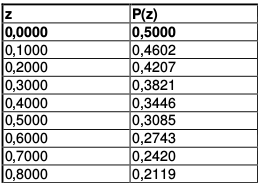
\includegraphics[scale=0.75]{res/table_loi_normale.png}
  \end{center}
  
  On voit que la valeur qui satisfait l'inéquation est $0.242 = P(z) \le 0.25$. Ceci donne une valeur de $z = 0,7$

  
  Le but est donc d'égaliser la partie à l'intérieur de la parenthèse :
		
  \[
      z = \frac{R - \mu_{D}}{\sigma_{D}}
  \]
		
  On isole $R$.
		
  \[
      R = \mu_{D} + z * \sigma_{D}
  \]
		
  On connait une autre formule de R :
		
  \[
      R = \mu_{D} + SS
  \]
		
   En égalisant ces deux dernières fonctions, on trouve la valeur du stock de sécurité :
		
  \[
      SS = z * \sigma_{D}
  \]
  
  Dans le cours, la valeur de $\sigma \approx 1,25 * MAD$ 
  
  \[
   SS = z * 1,25 * MAD
  \]
  
  Le MAD est ici au maximum de 4.
  
  \[
   SS = 0,7 * 1,25 * 4 = 3,5
  \]
  
  Notre stock de sécurité est donc 4 unités pour avoir une probabilité de rupture de 25\% maximum.

\end{solution}


\section{(2 points)}
  Expliquer, en moins de 5 lignes, quelle est la logique sous-jacente au calcul MRP.

\begin{solution}

  L'objectif du MRP est de planifier les ordres de commandes et/ou de production. La logique sous-jacente est une logique d'extrapolation. J'extrapole l'évolution du stock disponible en tenant compte de mon stock actuel, des besoins futurs et des livraisons futures. Sur cette base, je détermine quand je serai en rupture (ou sous le niveau acceptable) et je planifie les commandes afin d'éviter ces ruptures.
\end{solution}


\section{(2 points)}
 Votre portefeuille contient probablement de l'argent. Il s'agit d'un stock. Quatre types de stocks ont été analysés a ucours : stock cyclique, de sécurité, etc. Imaginez que cet argent constitue un stock cyclique. Expliquez la ou les raisons qui auraient induit ce type de stock. Expliquez aussi comment ce stock cyclique pourrait être réduit à zéro.

\begin{solution}
 Si cet argent constitue un stock cyclique, c'est qu'il y a un coût fixe dans le système et que je veux éviter de payer ce coût fixe trop souvent. La raison peut être simplement que je veux éviter d'aller au \og{} point d'argent \fg{} ou à la banque (coût fie lié au déplacement et au temps nécessaire) trop souvent.
 
 Eviter ce stock revient à trouver une solution qui me permet d'avoir de l'argent chaque fois que j'en ai besoin.
 
 Une première solution serait de réduire le coût fixe. Par exemple, avoir un \og{} point d'argent \fg{} très proche afin de pouvoir y aller souvent. Mais ceci ne réduit pas à zéro le stock cyclique.
 
 Une solution idéale serait d'avoir une carte me permettant de payer chaque fois que nécessaire (bancontact ou carte de crédit).
\end{solution}


 \section{(2 points)}
 
 Votre session d'examen constitue un projet. Vous l'avez planifiée et avez décidé de commencer toutes les tâches au plus tard. A quelle(s) tâches allez-vous accorder plus ou moins d'attention et pourquoi ?

\begin{solution}
 Ayant planifié toutes les tâches au plus tard, toutes sont maintenant susceptibles de retarder le projet. Je devrai donc acoorder la même attention à toutes les tâches, qu'elles soient critiques ou non.
\end{solution}

\end{document}
